\section{Purpose, scope and operating workflow}

\subsection{What Percepta produces}

Percepta is a desktop application for transforming an ordinary raster image into a structured RGB pattern. The output is deliberately dual in character. At close range, the observer sees a geometric construction: coloured stripes, dots or a spiral. At a larger viewing distance, or after reducing the image on screen, the same construction is spatially averaged and the source image becomes legible again.

The software therefore does not aim to imitate the source at every pixel. Instead, it preserves local red, green and blue contributions through the \emph{coverage} of three independently rendered structures. In a bright red region, the red structure occupies a larger fraction of the local pattern cell. In a neutral bright region, red, green and blue structures overlap strongly and the area tends towards white. In a dark region, little geometry is drawn and the background remains visible.

The intended uses include:

\begin{itemize}
  \item creating optical-illusion portraits and graphic artwork;
  \item producing animated transitions between obvious geometry and image reconstruction;
  \item exploring spatial vision, colour mixing and halftoning principles;
  \item preparing high-resolution raster or vector compositions for screen and print.
\end{itemize}

\begin{principlebox}
Percepta converts \textbf{intensity into geometry}. It does not merely recolour pixels or overlay a fixed screen. The source controls local stripe width, dot radius or spiral thickness separately in the red, green and blue channels.
\end{principlebox}

\subsection{Document scope}

This manual provides a complete operational and mathematical description of the current application. It explains the user interface, preprocessing, rendering families, parameter semantics, adaptive defaults, density animation, export and the perceptual basis of the illusion.

The equations describe the rendering model at the level needed to understand and reproduce its behaviour. A concrete implementation may use equivalent discrete formulations, cached intermediate images, vector paths or antialiased raster primitives. Consequently, two valid implementations can differ by subpixel edge placement while obeying the same model.

\subsection{Main interface}

Figure~\ref{fig:interface} reconstructs the application layout from the supplied interface captures. The exact dimensions adapt to the display, but the functional organisation remains the same.

\begin{figure}[H]
  \centering
  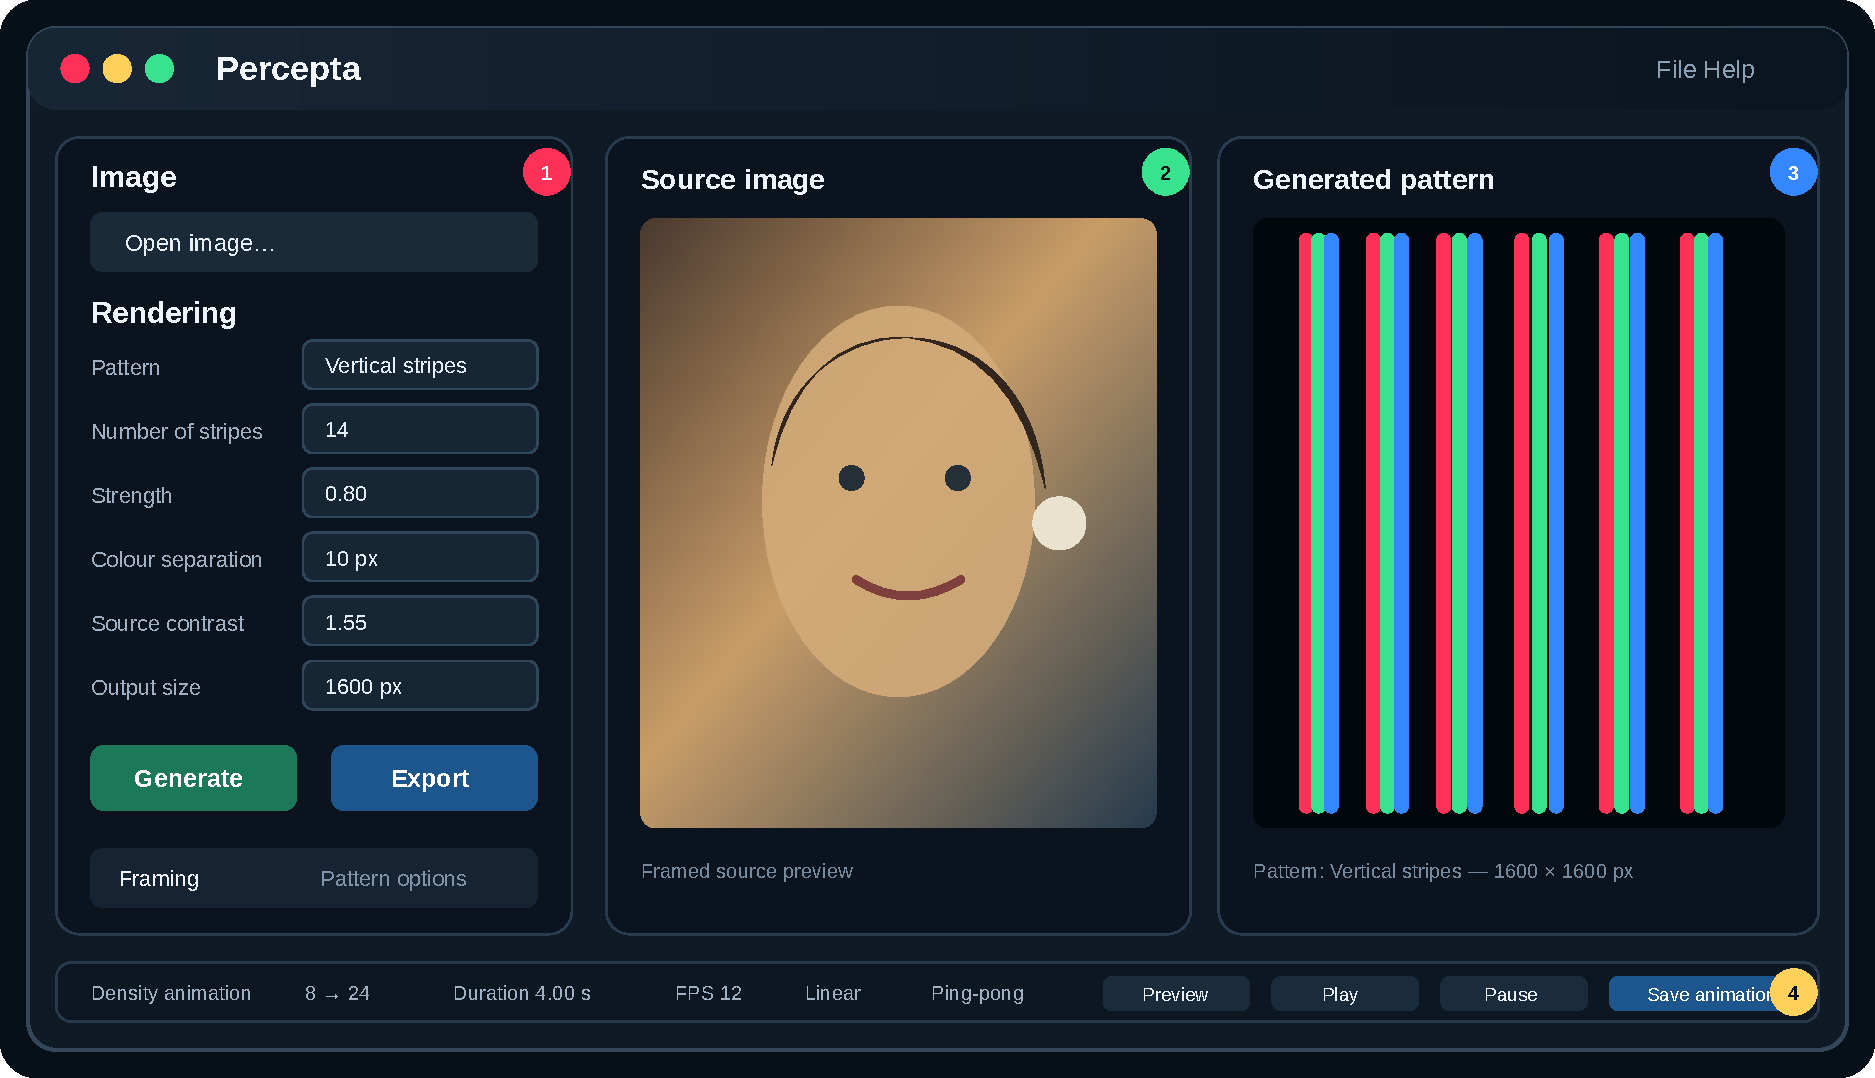
\includegraphics[width=0.92\textwidth]{build-assets/interface-overview.pdf}
  \caption{Percepta interface: (1) input and rendering controls, (2) framed source preview, (3) generated pattern preview, and (4) density animation controls.}
  \label{fig:interface}
\end{figure}

\subsubsection{Input and rendering panel}

The left panel contains the global workflow:

\begin{enumerate}
  \item \control{Open image...} loads the source.
  \item \control{Pattern} selects one of the six renderers.
  \item The density field changes its label and unit according to the renderer.
  \item \control{Strength}, \control{Colour separation}, \control{Source contrast} and \control{Output size} set common behaviour.
  \item \control{Generate} refreshes the output.
  \item \control{Export} writes the current result to a supported format.
\end{enumerate}

The two lower tabs separate geometric framing from options that apply only to the chosen pattern. This avoids displaying irrelevant controls and makes it clear which settings are global and which are renderer-specific.

\subsubsection{Source and generated previews}

The source preview is not necessarily the original file as loaded. It represents the result of crop, zoom, pan and rotation. This is the exact composition passed to the encoder. The generated preview shows the geometric output and reports the active pattern and output dimensions.

A useful evaluation habit is to inspect the generated result in three ways:

\begin{itemize}
  \item at full size, to judge edge quality and the visual character of the geometry;
  \item at an intermediate zoom, to see whether pattern and image coexist;
  \item as a small thumbnail, to judge reconstruction.
\end{itemize}

\subsection{Recommended operating sequence}

The following sequence minimises unnecessary recalculation and makes parameter interactions easier to understand.

\begin{enumerate}[label=\textbf{Step \arabic*.}]
  \item \textbf{Choose a suitable source.} Begin with an image having a clear subject, useful tonal range and limited clutter.
  \item \textbf{Set the output aspect ratio.} Select the crop before fine positioning.
  \item \textbf{Frame the subject.} Use zoom, pan and rotation until the source preview is satisfactory.
  \item \textbf{Choose the pattern family.} Select a line, halftone or spiral structure according to the intended visual character.
  \item \textbf{Generate at reference settings.} At 1600 px, use the pattern defaults in Table~\ref{tab:defaults} before making large changes.
  \item \textbf{Adjust density first.} Density determines the fundamental spatial scale and has the largest effect on recognisability.
  \item \textbf{Adjust Strength and contrast.} Use them to recover tonal separation without clipping.
  \item \textbf{Add colour separation carefully.} Coloured fringes are attractive, but excessive displacement breaks local RGB averaging.
  \item \textbf{Test at distance.} Zoom out or physically step back.
  \item \textbf{Increase output size for export.} Adaptive defaults preserve approximate apparent density, but the final result should still be checked.
\end{enumerate}

\begin{tipbox}
For a first portrait, use Vertical stripes at 14 stripes, Strength 0.80, Colour separation 10 px, Source contrast 1.55 and Output size 1600 px. Then compare the same framing with Halftone at 12 px and Spiral stripes at 19 px.
\end{tipbox}

\subsection{Pattern overview}

\begin{figure}[H]
  \centering
  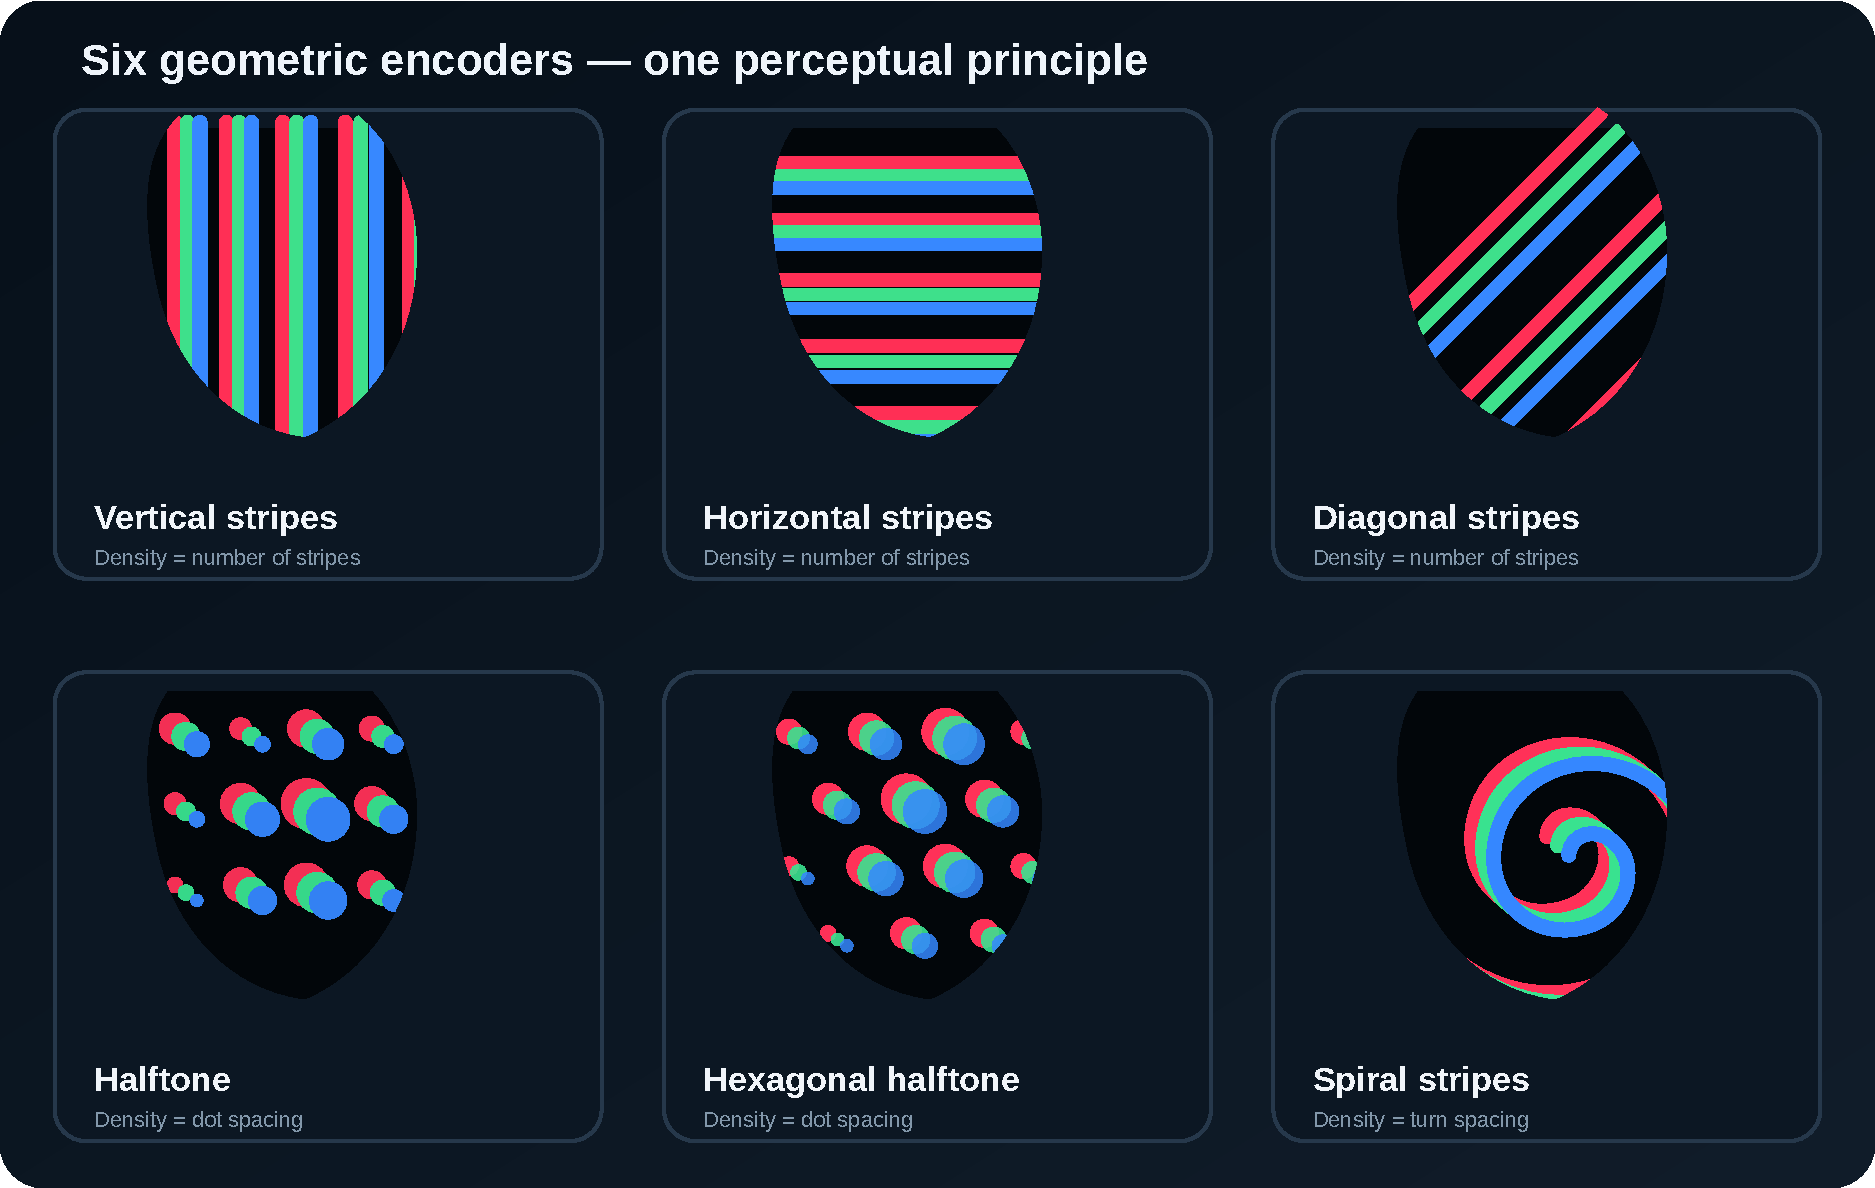
\includegraphics[width=0.92\textwidth]{build-assets/pattern-gallery.pdf}
  \caption{The six renderer families. The illustrations reproduce the visual logic of the supplied Percepta examples rather than a specific source photograph.}
  \label{fig:gallery}
\end{figure}

The line renderers use one-dimensional carriers whose local visible width changes with image content. The two halftone renderers sample on two-dimensional lattices and encode intensity as dot size. The spiral renderer follows a single continuous polar path and varies its local thickness.

These families share the same RGB decomposition and additive composition, so the controls remain conceptually consistent even though their density units differ.


